
\medskip

%Lors de son déménagement, Allan doit transporter son réfrigérateur dans un camion, Pour l'introduire
%dans le camion, Allan le pose sur le bord comme indiqué sur la figure. Le schéma n'est pas à l'échelle.
%
%\begin{center}
%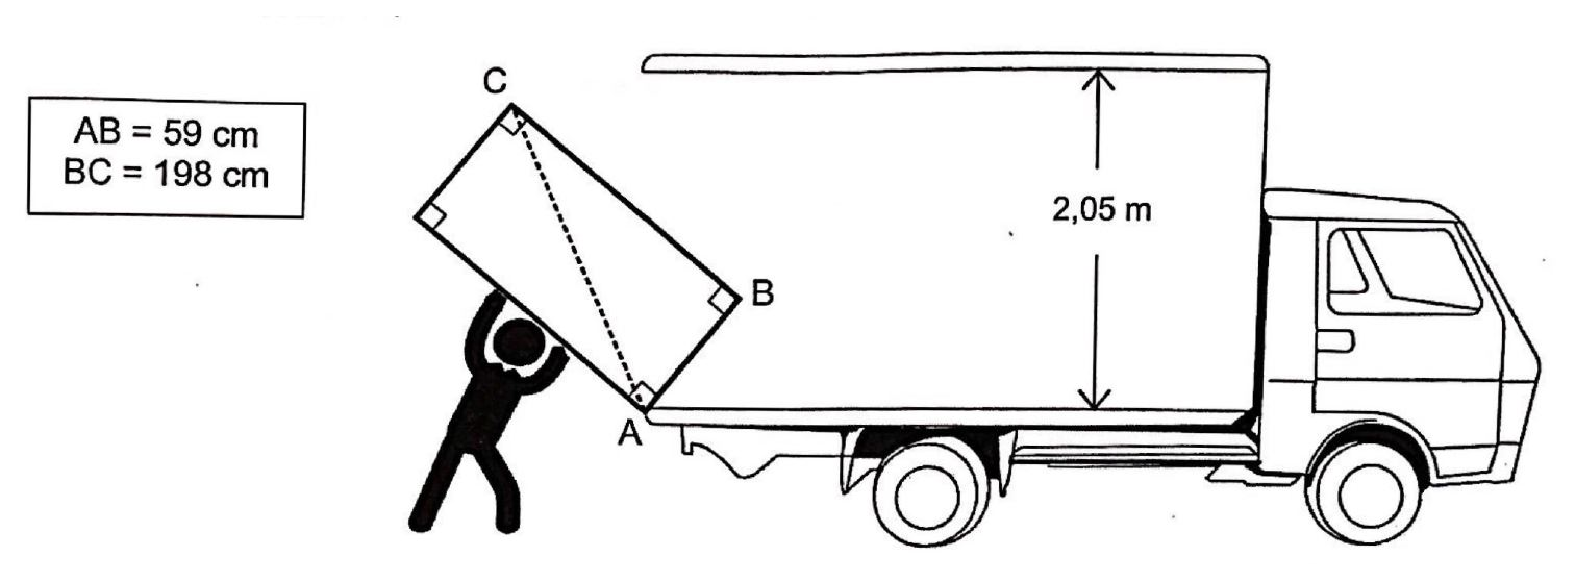
\includegraphics[width=12cm]{demenagement}
%\end{center}
%
%\smallskip
%
%Allan pourra-t-il redresser le réfrigérateur en position verticale pour le rentrer dans le camion sans
%bouger le point d'appui A ? Justifier.
Dans le triangle ABC rectangle en B, le théorème de Pythagore s'écrit :

$\text{AC}^2 = \text{AB}^2 + \text{BC}^2 = 59^2 + 198^2 = \np{3481} + \np{39204} = \np{42685}$.

Donc $\text{AC} = \sqrt{\np{42685}} \approx 206,6$~cm soit $2,066$~m. Allan ne peut redresser le réfrigérateur en position verticale.

\vspace{0,5cm}

